
\documentclass[technote]{IEEEtran}

\usepackage{alltt} 
\usepackage{graphicx}
\usepackage{amsmath}
\usepackage{amssymb}
\usepackage{amstext}
\usepackage{hyperref}

\everymath{\displaystyle}
\hypersetup{pdfborder = {0 0 0}}

\title{Evaluation of SMOTE and drift detection methods for data streams}
\author{R. Anderson, K. Chen and S. Jin}
\date{}

\begin{document}
\maketitle

\begin{abstract}
Classification of data streams with class imbalance is a challenging field that is not yet fully researched, especially when concept drift is considered. We propose a new method for classification of rare classes in an imbalanced stream with concept drift, through using SMOTE to oversample minority classes in data streams. We evaluate the performance of this approach without a drift detector, and with PHT and ADWIN, through using synthetic data streams generated through MOA with varying degrees of drift and imbalance. We also test our approaches against a real world dataset.

We show that both drift detectors are comparable when used in a streaming environment with imbalanced data. Our results show promise in terms of recall and F-Score but highlight potential issues in terms of time complexity from use of SMOTE. 
\end{abstract}

\section{Introduction}
In recent years, researchers have drawn attention to data stream mining in the field of data mining, as dramatic increases in computing power make it feasible. Problems with imbalanced datasets (those with a skewed class distribution, with majority classes and minority classes) have been well researched in the static data mining context. Imbalanced data stream exists in many applications such as network traffic data and credit card transactions. They suffer from concept drift, which refers to the underlying class distribution of data streams potentially changing over time. 

Concept drifts have been studied in depth over recent years. An example of concept drift is online shopping customer preferences changing over time. A drift can happen abruptly or gradually. To solve the problem of concept drift, predictive models need to be updated, which is also called online adaptive learning. Concept drift is difficult to detect because the detector may be confused with noise and outliers. There are very few studies combining the two problems of concept drift and imbalanced data stream. One representative paper is �A General Framework for Mining Concept-Drifting Data Streams with Skewed Distributions \cite{gao}�, in which Gao proposed a framework applying both under-sampling and ensemble techniques demonstrating better prediction performance.

We will explore a method that will combine concept drift detection and sampling underlying data to contribute to the area of classification of imbalanced data in data streams with concept drift. We will examine the effectiveness of concept drift detectors in imbalanced data; examine whether SMOTE \cite{SMOTE}, a method that oversamples minority classes can assist with classification performance; and test the time and memory use of our method against cases not using our method, to measure the feasibility of its use in data streams. 

MOA and Weka libraries include a lot of ready-to-use algorithms for stream data mining. In our experiment, we use MOA and WEKA�s API to interact with MOA�s stream mining capability and SMOTE�s sampling capability. We have modified some synthetic data stream generators to provide 3 different levels of desired class imbalance proportion: 0.01, 0.1, 0.5. For each data stream generator we use 30 different seeds, which will ensure that our experiment result is not due to random chance and our result could be re-produced by setting the same seed; we have prepared 3 different concept drift detection methods to be used along with the HoeffdingTree base learner; we have set up a test suite to record some evaluation metrics for every possible combination setting among different dataset, class imbalance ratio, concept drift detection methods while running our experiment with and without SMOTE sampling presented.

Beyond this, we also test our technique on the Electricity dataset, a well-known real world dataset that can be used to test the effectiveness of our classification.

This paper is organized as follows: the next section briefly presents the related work we have drawn on for our research. The Problem Description section will detail the scope of our work. The Methodology section discusses our experimental approach in detail, and attempts to explain and justify how we have conducted our research. The Results section presents findings from our experiments - first those testing our hypotheses with the synthetic data, and then testing our approach on the Electricity dataset. We propose several extensions to our work in the next section, Future Work. Finally, we conclude the paper by summarising our results and findings.

\section{Related Work}

Various useful literature reviews summarise the challenges and approaches to tackling classification in data streams with concept drift and class imbalance. We particularly recommend \cite{gam04}, who provides a thorough description of the field. Hoens et al. \cite{hoe12} provide an excellent summary of the latest research in the area as well.

A few papers discuss their approaches to solve the imbalance problem for concept-drifted data streams. Classifier ensembles along with sampling approaches are solutions presented in \cite{classifier_ensemble} and \cite{gao}. Gao has shown that reconstructing a model on new data reduces expected error theoretically and experimentally. His proposed algorithm employs both sampling and ensemble techniques to generate reliable probability estimates and reduce misclassification error rates. However, these two methods have used different sampling techniques. SMOTE \cite{SMOTE}, SERA \cite{SERA}, MUSERA \cite{musera}, REA \cite{rea} and Learn++SMOTE \cite{LEARN} are over-sampling based approaches. 
				
Generally, classifier ensemble is believed to perform better on the imbalanced data stream. Ensembles consist of many components (typically different models or learners) which are combined by voting or averaging the outcomes from each component. Ensemble methods can often improve the accuracy of a single classifying algorithm. A drawback is the increased memory and time requirement. We have sought an alternative approach to this method.

In �A Double-Ensemble Approach for Classifying Skewed Data Streams�, Zhang et al. \cite{zhangstatic} proposed a clustering-sampling based ensemble algorithm with weighted majority voting for learning skewed data streams, he uses k-means clustering algorithm for selecting minority instances to represent minority class, the centroid of each cluster is used as an instance for the class. He also proposes using a flexible approach that can alternate between learners, roughly based on the imbalance of the stream in \cite{zha12}.
				
We use an implementation of Hoeffding Trees through our research, as initially described by Domingos and Hulten \cite{dom00}. In \cite{paz14} , Andrea et al. avoided sampling by using Hellinger Distance Decision tree (HDDT\cite{paz14} as a base learner for data streams, which showed superior performances in terms of prediction accuracy, recall rate, computational time and resources. HDDT theory derives a new decision tree splitting criteria based on Hellinger distance that is skew insensitive.

In this paper we test the performance of two drift detectors ADWIN - an adaptive windowing approach \cite{adwin} and PHT - a sequential approach \cite{PHT}. A study done by Goncalves et al. evaluated different drift detection methods (including ADWIN, PHT, DDM) on a variety of gradual and abrupt streams \cite{gonc14}.  

\section{Problem Description}
The problem we are interested in is the binary class classification problem in data streams with imbalanced classes and underlying concept drift. We evaluate the effects of applying a sampling method (SMOTE) that is effective in the static context to the streaming environment by combining it with drift detectors (ADWIN and PHT) and a single base learner (Hoeffding tree). We investigate how these different hybrid approaches perform on datasets with different characteristics such as data with gradual drifts, abrupt drifts, and varying levels of class imbalance. The performance measures of interest to us include memory usage, runtime, overall accuracy, recall, precision and F-score.

Our hypotheses are:
\begin{enumerate}
\item Applying sampling techniques to drift detectors will greatly improve the performance of Hoeffding Tree classifiers for datasets with high and moderate degrees of class imbalance compared to drift detectors without sampling.
\item Applying more layers of complexity (i.e. sampling, drift detection) to the base learner will increase the time and memory requirements, but will not always guarantee better performance.
\item There is no statistically significant difference in accuracy or f-score between using different drift detectors.
\end{enumerate}

\section{Methodology}

Our experimental framework is as follows:\\
(1) Each type of synthetic stream is generated 30 times using different seeds.\\
(2) Testing is performed on the learner before learning.\\
(3) If the SMOTE flag is set perform SMOTE and randomization, otherwise train on a block of 2,000 instances.\\
\\SMOTE:
\\Each block of 2,000 instances is passed to the SMOTE filter to be sampled.\\
\\Randomization:\\
The resulting instances generated from SMOTE are randomized, and a random sample of 2,000 instances are used to train the learner.\\
\\
Here the learner may refer to the Hoeffding tree, or the Hoeffding tree combined with ADWIN or PHT. Evaluation on the real dataset also follows the same procedure, except the first step is replaced with preparation of the data stream.

\begin{figure}[t]
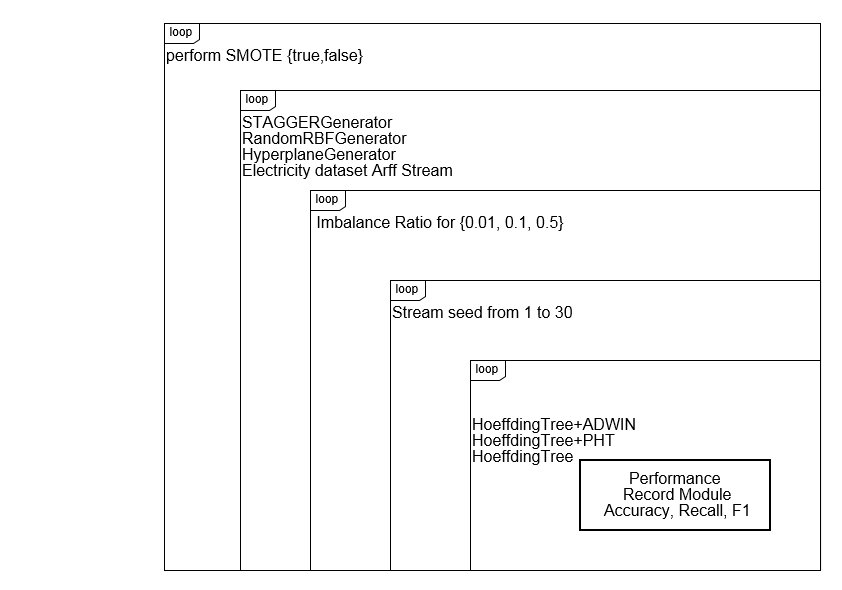
\includegraphics[width=0.48\textwidth]{1024}
\caption{Diagram of experimental framework}
\end{figure}

We used implementations provided by the MOA and WEKA packages to run our experiments.

We have chosen to analyse the performance of our methods using both synthetic and real world datasets. Synthetic datasets allow us to control various properties of the stream that we are interested in such as the position of drift, the speed and severity of drift as well as the noise ratio and class balance. This enables us to analyse how the combinations of algorithms perform under different conditions. We generated 9 different types of streams (all combinations of 3 levels of class balance with 2 speeds of drift as well as the no drift case), each with a total stream size of 1,000,000 instances (summarized in the table below). We used 3 different types of learners: Hoeffding tree, Hoeffding tree with ADWIN as a drift detector, and Hoeffding tree with PHT. To evaluate the costs and benefits of SMOTE as a technique to cope with class imbalance in streams, we compare different combinations of learners and stream types with and without SMOTE.

\begin{figure}[b]
\begin{tabular}{lll}
\hline
Class balance \% & Drift type & Generator              \\
\hline
1                & Abrupt     & STAGGER                \\
10               & Abrupt     & STAGGER                \\
50               & Abrupt     & STAGGER                \\
1                & Gradual    & RandomRBFGeneratorDrift\\
10               & Gradual    & RandomRBFGeneratorDrift\\
50               & Gradual    & RandomRBFGeneratorDrift\\
1                & No Drift   & STAGGER                \\
10               & No Drift   & STAGGER                \\
50               & No Drift   & STAGGER                \\
\hline \\
\end{tabular}
\caption{Synthetic stream types}
\end{figure}

We chose to examine 3 different levels of class balance: 1\%, 10\% and 50\% (which we refer to as very imbalanced, imbalanced and balanced throughout the paper). The percentage of class balance describes the proportion of instances in the whole dataset that are in the minority class. For example 50\% class balance means that 50\% of all instances in the stream are in the minority class - this is the fully balanced stream. 

We construct our synthetic datasets in a way such that the instances of the minority class are approximately evenly distributed and the class balance level remains constant throughout the stream. 

We also chose to examine different speeds of drift: abrupt drift, gradual drift in addition to streams with no concept drift (as a comparison). Abrupt drift describes cases where the change in concept occurs suddenly, whereas for gradual drift the change occurrs more slowly accross a longer period of time.

We chose to use the STAGGER dataset for generating streams with abrupt drift as it has been commonly used in other studies that deal with concept drift and may make our results more comparable to previous studies. The STAGGER dataset has 3 categorical attributes (shape, color and size), each with 3 possible values. The concepts are in the form of boolean functions relating to the 3 attributes. The functions are (1) color = red AND size = small, (2) color = green OR shape = circle, and (3) size = medium OR size = large. 

As the default STAGGER generator in MOA does not generate instances according to some balance level we modified the STAGGERGenerator in MOA to generate streams with 3 levels of class balance. Our method for generating an imbalanced STAGGER stream is as follows: First we balance the classes by setting the balance option in the generator, then we sample the minority class with probability $\frac{w}{1-w}$, where $w$ is the percentage of class balance {[}0 , 0.5{]} to give the level of class balance we require.

To simulate an abrupt drift we joined two streams using the ConceptDriftStream generator provided by MOA and specified the drift position to be at the 300,000th instance with an angle of 90 degrees. The angle determines the level of abruptness of the change which is modelled by a sigmoid function, we have chosen to use an angle of 90 degrees to simulate a very abrupt change in concepts.

The modified STAGGER generator was also used to generate the streams without concept drift for ease of comparison with the abrupt stream.

To generate streams with gradual drift at various balance levels we used a modified version of the RandomRBFGeneratorDrift from MOA which generates random radial basis concepts with drift. We modify the RandomRBFGeneratorDrift in a similar way to the method described for the STAGGER generator. The parameters we used were 10 attributes, 3 centroids (all centroids with drift), and a speed of 0.01 to simulate a stream with gradual concept drift. The speed describes the speed at which the centroids are moved and the value of 0.01 was chosen to provide a slower gradual drift in contrast to the abrupt drift stream. The number of attributes and drifting centroids were chosen to provide a more challenging concept for the Hoeffding tree to learn. Sample runs with 2 drifting centroids on a Hoeffding tree learner done prior to the experiments showed that the learner performed almost optimally (with accuracy reaching above 90\%) so a higher value was chosen.

We used the SMOTE filter implemented in WEKA. The parameters we used were 5 nearest neighbors, and a variable percentage value. This percentage value is the percentage of SMOTE instances to create, and we compute this value according to the number of instances in the minority and majority class. We chose to increase the minority class percentage so that the number of minority and majority instances in the 2,000 instance block is the same.
We passed instances in blocks of 2,000 to the SMOTE filter because we felt this could be an appropriate size to allow feasible processing time and the ability to capture enough minority instances (to sample from). However this parametization needs further investigation. As SMOTE adds the synthetically generated isntances to the end of the list, this requires a randmoization procedure to ensure the instances are randomly distributed so the drift detector does not detect many false positives.

We evaluated the classifier using a blocking prequential approach. We test the learner using blocks of 2,000 instances before the learner is trained using these instances. This approach seems more fitting to our experimental design than testing using a Holdout dataset (due to the nature of concept drift), the single instance test-then-train approach, or the prequential method with a decay function. 

To evaluate our learner we use accuracy, recall, precision, f-score, memory and runtime. Accuracy is a standard measure of classification performance, but is not a good measure for classification of minority classes because the contribution to the accuracy score decreases as the class becomes rarer. In these scenarios recall and precision may be better indicators than overall accuracy alone. F-score is a way of combining recall and precision into a single value (a f-score close to 1 is often viewed as a better score).
The memory is the memory of the learner - the Hoeffding tree. The runtime includes the timing of the SMOTE procedure, randomization of instances (post SMOTE) and the training of the classifier. Time used during instance generation, stream preparation and testing were ignored.

We used the default parameters for PHT as implemented in MOA. For ADWIN, we used the default maximum window size of 32 instances and a delta of 0.002. Adjusting the maximum window size to the same size as the SMOTE block (2,000 instances) did not appear to provide any improvements in the accuracy, recall or runtime when we tested this against our synthetic datasets. 

For the Hoeffding tree learner, information gain was used as the spliting criterion.

We also examined the performance of a real dataset (the Electricity dataset) provided by Gama (cite something). This dataset has 8 attributes and a total of 45,312 instances. There are 2 classes (up, down) which reflect the price changes of electricity prices in New South Wales compared to the average price in the last 24 hours. This dataset has 40\% of total instances in one class, and 60\% in the other class. As this dataset does not show much class imbalance we modified this dataset by undersampling the `up' class to produce 5\% and 10\% class balance and tested the algorithms on the skewed datasets as well as the original dataset.

Finally we analysed these results by comparing 95\% confidence intervals, mean and maximum scores for accuracy, f-score, runtime and memory usage.

\section{Results}

In this section, we will present the aggregated results of our experiments for our synthetic datasets and discuss each of our hypotheses in turn. We will continue on to showing results for the Electricity dataset (accessible from $http://www.inescporto.pt/$\textasciitilde$ jgama/ales/ales_5.html$), to give an idea of how our approach may work on real world data.

\subsection{Synthetic Datasets}

For our synthetic datasets, we ran experiments 30 times for every combination of factors, on streams with 1 million instances generated. We present the mean of those experiments along with a 95\% confidence interval given the variance in our experimental results. In graphs following, error bars show the range of this interval (though note that some experiments were so consistent that these error bars are almost invisible). 

The data-level factors we varied across these experiments were: 
\begin{itemize}
\item stream generators, with levels '\textbf{No CD/drift}' (STAGGER), '\textbf{Gradual}' drift (RBFGenerator) and '\textbf{Abrupt}' drift (STAGGER)).
\item class-balance ratio, with levels '\textbf{Balanced}' (1:1), '\textbf{Imbalanced}' (1:9) and '\textbf{Very Imbalanced}' (1:99).
\end{itemize}

The learning-approach factors we varied across these experiments were:
\begin{itemize}
\item sampling method, with levels '\textbf{SMOTE}' and '\textbf{No SMOTE}'.
\item drift detection method, with levels '\textbf{ADWIN}', '\textbf{PHT}' (Page-Hinkley Test) and '\textbf{No DDM}' (no drift detection).
\end{itemize}

Through our experiments in this section, we have chosen to focus on four evaluation measures: memory, runtime, accuracy and F-Score. Memory refers to model size at the end of the experiment. This is affected heavily by drift detectors, which regularly may choose to dispose of a model after detecting drift. Runtime refers to total time to run the experiment, excluding stream generation and evaluation of the model. Accuracy refers to the proportion of instances correctly classified. F-Score is a weighted average of recall (the true positive rate) and precision (positive predictive value). This measure discourages maximimising accuracy by defining all as the majority class in an imbalanced dataset, and values intelligent predicting of the minority class. We do not expect SMOTE to outperform SMOTE-less experiments in accuracy, but if it is effective, we can expect to see a superior F-Score.

In our tabulated results (which can be found at the end of this document), for each set of factors we are comparing, we have put the best result in bold. This may involve some or all comparisons when the 95\% confidence intervals we have used overlap.

\subsubsection{Impact of drift detectors upon classification}

To test our hypothesis that there is no significant difference in accuracy between drift detectors, we have chosen to examine our streams with gradual and abrupt drift with balanced and very imbalanced data(Fig 3 and 4), and include results for the no drift and imbalanced situations in our tabulated results (Fig 5). 

\begin{figure}[ht]
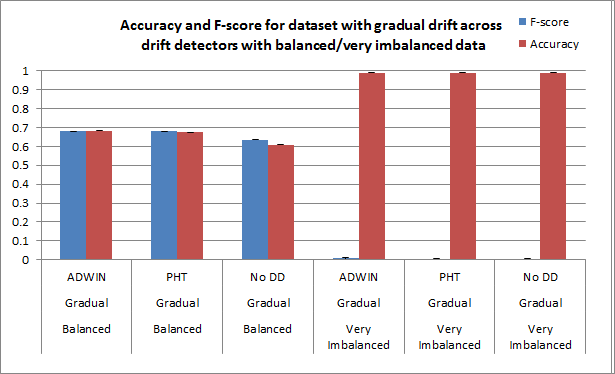
\includegraphics[width=0.48\textwidth]{GDriftGrad.png}
\caption{Evaluation measures for drift detectors with gradual drift}
\end{figure}

Our gradual stream had ten variables, making it more difficult to classify correctly than the STAGGER-based streams that only had three. We can see for balanced data that ADWIN and PHT worked similarly well, with having no difference in F-Score, and ADWIN being marginally better for accuracy. In the very imbalanced situation, ADWIN had a slightly better F-score while PHT had a slightly improved overall accuracy. Both worked significantly better than having no drift detection.

\begin{figure}[h]
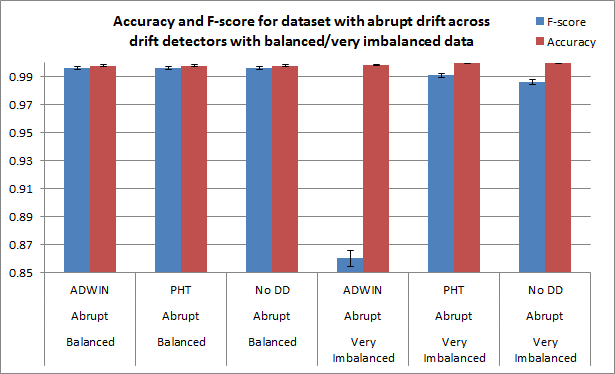
\includegraphics[width=0.48\textwidth]{GDriftAbr.png}
\caption{Evaluation measures for drift detectors with abrupt drift}
\end{figure}

With the abrupt datastream, no significant difference in accuracy nor F-score could be seen between any type of drift detector until the data became very imbalanced. At this point, PHT outperformed ADWIN very significantly for F-Score, and marginally in accuracy. Having no drift detector did. It may be due to ADWIN changing its model too regularly to be able to clearly classify the rare class, which it sees few instances of. A small number of misclassifications of a rare class can lead to a large impact on an F-score as well.

\begin{figure*}[h]
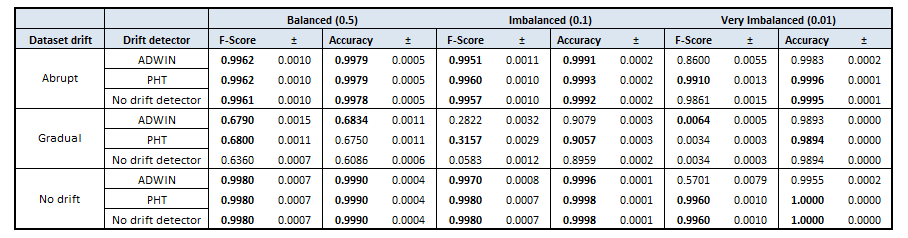
\includegraphics[width=\textwidth]{DriftTable.png}
\caption{F-Score and Accuracy for combinations of drift, drift detector and balance with no SMOTE}
\end{figure*}

Analysing our table, we can see that across all testing circumstances, PHT and ADWIN are often indistinguishable, and trade off the top-spot for different measures under different circumstances. There is only one combination where either work much worse than having no drift detection (F-score for ADWIN with abrupt drift.) It would be difficult to claim that either drift detector is strictly better, and both regularly work better than no drift detector in terms of classification measures, so our experiments uphold our hypothesis.

\subsubsection{Impact of SMOTE upon classification}

To test our hypothesis that applying sampling techniques to drift detectors greatly improves the performance of classifiers for imbalanced/very imbalanced datasets, we have compared results of experiments with and without ADWIN for gradual and abrupt drift (Fig 6 and 7), and include this and the data for the case with no drift in Fig 8.


\begin{figure}[h]
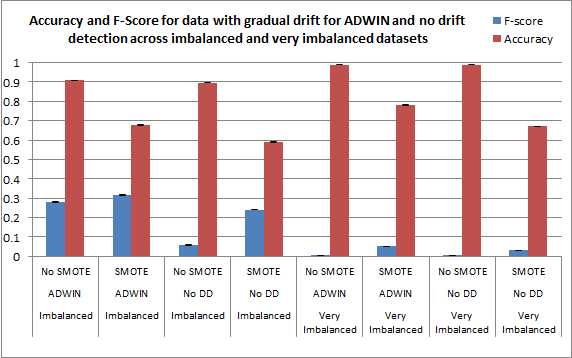
\includegraphics[width=0.48\textwidth]{GSMOTEGrad.png}
\caption{Evaluation measures for classification with SMOTE with gradual drift}
\end{figure}

With the gradual data stream, we can see a dramatic difference between the performance of the SMOTE and non-SMOTE runs across all combinations. Accuracy is significantly worse for all measures while F-Score is significantly better. This suggests that the classifiers are correctly classifying more of the minority class at the cost to overall accuracy, which matches what we would predict. 

\begin{figure}[h]
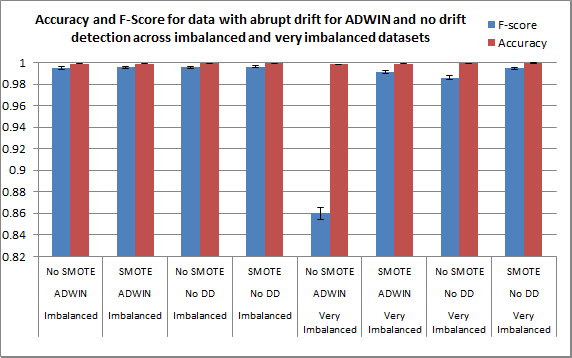
\includegraphics[width=0.48\textwidth]{GSMOTEAbr.png}
\caption{Evaluation measures for classification with SMOTE with abrupt drift}
\end{figure}

With the abrupt data stream, we cannot see as dramatic a difference. The learner with no drift detector manages well on this stream, and so the inclusion of a drift detector does not make a significant difference. As Figure 8 shows, there is no significant difference in the classification accuracy on any of these methods. With very imbalanced data, using SMOTE leads to a slight improvement in F-Score with no drift detector, and a significant improvement when using ADWIN. SMOTE has worked with ADWIN to improve in classifying the rare class in this instance.

\begin{figure*}[h]
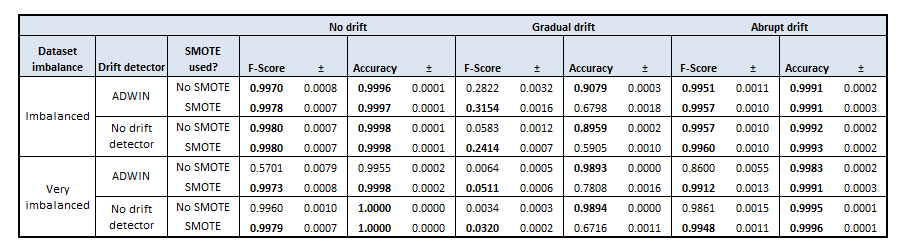
\includegraphics[width=\textwidth]{SMOTETable.png}
\caption{F-Score and Accuracy for combinations of drift, balance, drift detector and sampling method}
\end{figure*}

Figure 8 shows that the simplicity of our no drift and abrupt drift streams lead to little distinction between the performance of SMOTE and no SMOTE, apart from with ADWIN in the very imbalanced circustance. However, the gradual drift results show that SMOTE consistently improves F-Score with and without a drift detector in place. This matches what we would expect, and shows that SMOTE does improve classification performance where F-Score is more important than accuracy.

\subsubsection{Impact of SMOTE and drift detectors upon cost}

To test our hypothesis that both drift detectors and sampling methods would increase the cost  of our analyses, we compared final model memory size and runtime at the end of our experiments across use of SMOTE and our three levels of drift detector. We investigated all of these for our imbalanced level of data (with a 0.1 rate of minority class instances), which we believe will be representative of the relationship. We have included tabulated data in Figure 13 and 14. 

\begin{figure}[h]
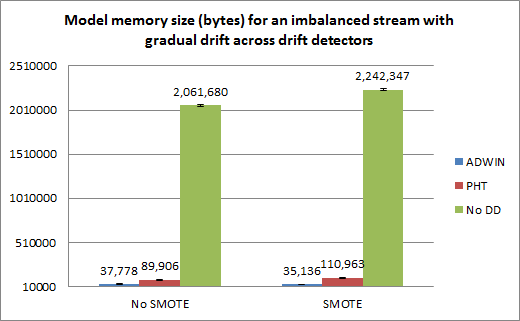
\includegraphics[width=0.48\textwidth]{GComplexityMemGrad.png}
\caption{Final model memory size for an imbalanced stream with gradual drift}
\end{figure}

In this case, we see the case with no drift detection dramatically larger than with two drift detectors. This makes sense - drift detectors replace a model once drift is detected, and so it is likely that the model is being regularly replaced for the cases with drift detection. The Hoeffding Tree grows dramatically to record the different examples it sees under gradual concept drift. This is exacerbated by the high dimensionality of this stream. It is larger with SMOTE, possibly as it tries to record more examples of both classes rather than focussing on the majority class.

PHT is statistically significantly larger with SMOTE, suggesting that the oversampling method is reducing the total number of drifts detected. This may be because it gives a consistent class ratio, or because our method of using SMOTE 'scrambles' data order to a small degree through resampling. It is interesting that SMOTE appears to affect PHT and ADWIN differently in this case.

\begin{figure}[h]
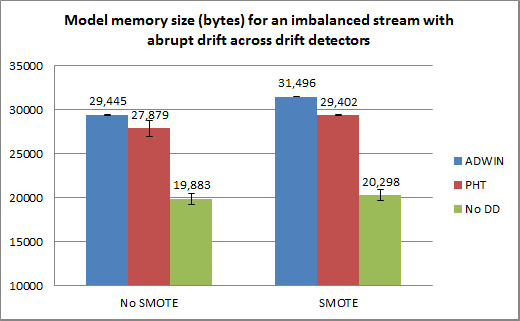
\includegraphics[width=0.48\textwidth]{GComplexityMemAbr.png}
\caption{Final model memory size for an imbalanced stream with abrupt drift}
\end{figure}

When looking at the abrupt drift stream, the case with no drift detection is much smaller than for the gradual drift stream - most likely as the tree must only record two variants of drift, and for much lower-dimensionality data. ADWIN and PHT are consistently sized. SMOTE results in slightly larger trees for the learners with drift detectors, but not concerningly so. This may be due to the reasons listed for the gradual stream.

\begin{figure}[h]
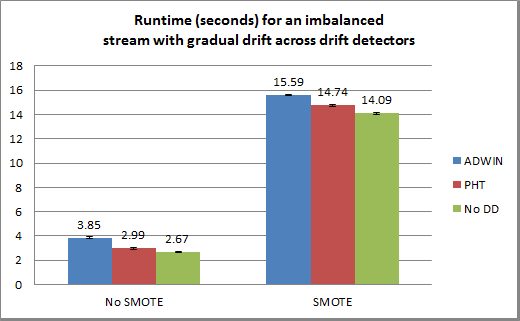
\includegraphics[width=0.48\textwidth]{GComplexityTimeGrad.png}
\caption{Runtime for an imbalanced stream with gradual drift}
\end{figure}

We see that for gradual streams, ADWIN runs more slowly than PHT, which runs more slowly than no drift detector. With SMOTE, the gradual stream takes significantly longer to run. This is likely due to the high dimensionality data - SMOTE uses k-NN, which suffers from the 'curse of dimensionality'. This provides an important insight into the limitation of this technique of analysis.

\begin{figure}[h]
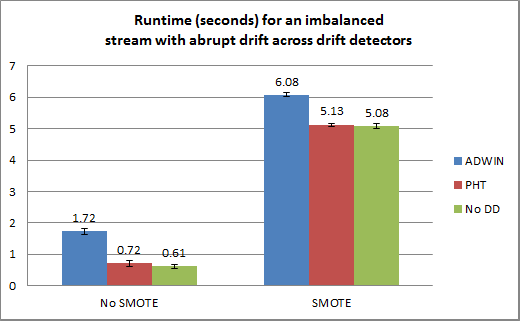
\includegraphics[width=0.48\textwidth]{GComplexityTimeAbr.png}
\caption{Final model memory size for an imbalanced stream with abrupt drift}
\end{figure}

We can see similar results in the abrupt stream to the gradual stream in terms of runtime. However, SMOTE runs in 4-5 times the length of time of non-SMOTE rathan than 6-8 times the length of time. This is due to fewer dimension in the STAGGER-generated data. ADWIN seems notably slower than PHT.

In terms of model memory, having no drift detector can potentially allow the size to balloon out, compared to having a drift detector. Presumably, if no drift is detected, models with drift detectors would be in danger of ballooning out as well. This may be why using SMOTE tends to lead to larger models - by interfering with a drift detector's ability to detect drift. However, imbalanced data may have false drift due to the chance of a rare class disappearing or becoming suddenly prevalent when no underlying drift exists. SMOTE would help maintain a level of accuracy over this time rather than restarting the model. Our hypothesis does not hold over memory - SMOTE may increase memory size somewhat, but drift detectors potentially reduce the memory size when using a Hoeffding Tree in the presence of drift.

In terms of runtime, drift detectors appear to be minorly detrimental. PHT seems to run very quickly in our experiments - almost as well as having no drift detector. ADWIN is a little more costly. Including SMOTE in the analysis obviously had very significant impact on time taken. This would be an important consideration when considering use of our method, and further studies would need to be conducted to see whether this would bar it from being a useful streaming tool. Low-dimensional data helps minimise the time difference. Further experiments could show that a smaller 'interval' of instances speeds up this approach suitably for a streaming context. The fundamental issue is SMOTE's exponential complexity, which will regularly lead to such increases in time taken for analyses. These findings support our hypothesis in regards to runtime. 

\begin{figure*}[h]
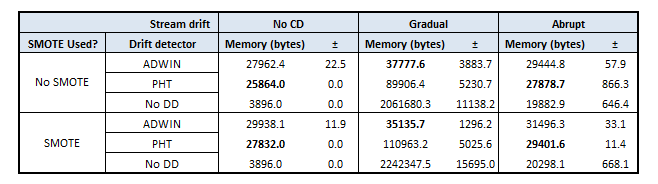
\includegraphics[width=0.8\textwidth]{ComplexityTableMem.png}
\caption{Model memory at end of run for sampling method, drift detector and stream drift for imbalanced data}
\end{figure*}

\begin{figure*}[h]
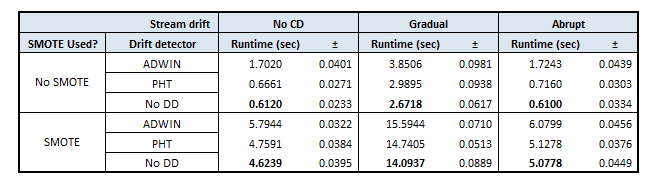
\includegraphics[width=0.8\textwidth]{ComplexityTableTime.png}
\caption{Runtime in seconds at end of run for sampling method, drift detector and stream drift for imbalanced data}
\end{figure*}

\subsection{Electricity Dataset}

To evaluate the quality of our approach against real world data, we analysed the Electricity dataset from the UCI repository. This dataset contains 45,312 instances of changes in the electricity price in an Australian Electricity Market (UP or DOWN) against eight relevant variables. As this is real world temporal data, and based on other studies, we expect some underlying drift to be present. Below, we show measures for accuracy, precision, recall and F-Score for this dataset. The original dataset has a class balance of 45:55. To make it more suitable to our interest in imbalanced datasets, we randomly sampled the minority class ('UP') to artifically create a dataset of class ratio 1:9 and 1:19. Below we show the results for the 1:9 imbalanced datasets across all levels of drift detection in Figure 15 and 16, and for all datasets in Figure 15. In the plots below, 'No DDM' refers to no drift detection method, and each combination of drift detector and sampling method is examined.

\begin{figure}[h]
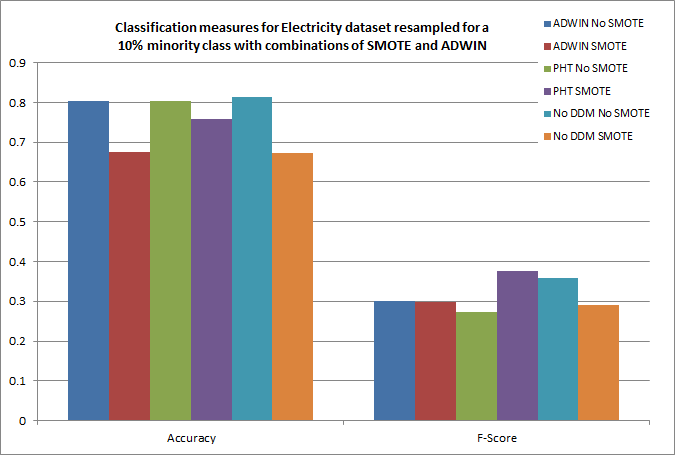
\includegraphics[width=0.48\textwidth]{GElecAccFScore.png}
\caption{Accuracy and F-Score for analysis of Electricity dataset}
\end{figure}

We can see that for our imbalanced data, accuracy was generally worse when using SMOTE but F-SCore was consistently equal or better. SMOTE with PHT appeared to be a very strong combination, for identifying the minority class. We can investigate further into the F-Score by looking at recall and precision for this analysis.

\begin{figure}[h]
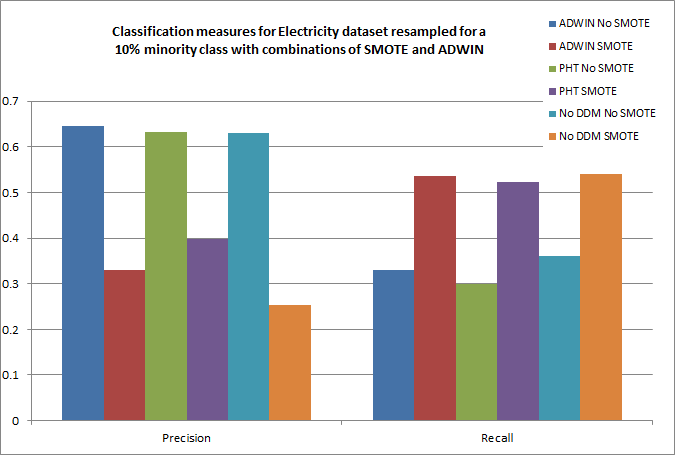
\includegraphics[width=0.48\textwidth]{GElecRecallPrecision.png}
\caption{Precision and Recall for analysis of Electricity dataset}
\end{figure}

This data shows the impact of SMOTE very effectively. SMOTE consistently and significantly improves recall across each level of drift detection. Meanwhile, it negatively impacts precision. The combined effect of this is generally to lead to an improvement in F-Score. This supports the use of SMOTE's utility in classifying minority classes.

\begin{figure*}[h]
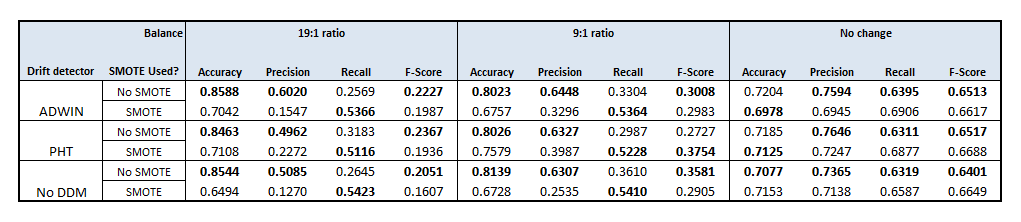
\includegraphics[width=\textwidth]{ElecClassTable.png}
\caption{Classification evaluation measures for Electricity data}
\end{figure*}

Examining the summary classification data in Figure 17, we can see that recall with SMOTE consistently was significantly better than without SMOTE for imbalanced data. The converse was true for precision and accuracy. With a 19:1 ratio of imbalance, the F-Score was superior for analysis without SMOTE. This may be because with such a small dataset, the model does not see enough instances of the minority class to properly classify it.

\begin{figure*}[h]
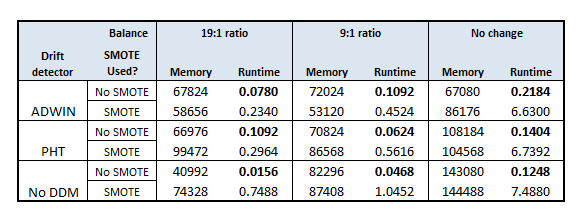
\includegraphics[width=0.7\textwidth]{ElecCostTable.png}
\caption{Cost evaluation measures for Electricity data}
\end{figure*}

Runtime for SMOTE was very poor for the unchanged data, but improves drastically as the dataset becomes more imbalanced. This is most likely because SMOTE will find Euclidean difference for every minority class point, which will be much more time-consuming in near balanced data. With no drift detection, using SMOTE came at a much larger runtime than without SMOTE. This difference is surprising and unexpected. Further experiments would be required to verify this result.

Memory usage was higher for models with SMOTE consistently, especially for drift detectors. This is likely due to SMOTE obscuring drift, and resulting in larger models being kept.

Overall, the data shows that SMOTE does effectively improve identification of the minority class in imbalanced data. It does come with a relatively large increase in runtime across all experiments, but this can be minimised by using it on very imbalanced data.

\section{Future Work}

Through our experiments, we chose an arbitrary value of 2000 as a block size to pass through SMOTE and then pass to drift detectors. This effects SMOTE runtime (smaller blocks would be better), SMOTE effectiveness at oversampling minority classes (larger blocks would be better) and drift detectors using the data (larger blocks obscure changes in the data). Repeating these experiments with a different block size could potentially show speed improvements without a significant loss in accuracy or F-Score. 

Further parameter tuning of our drift detection methods could also provide performance gains. We potentially lose a lot of information about the underlying characteristics of concept drift in a stream through applying SMOTE, which could be investigated as a piece of further work.

As SMOTE runs with K-NN, it is limited by the complexity of the Euclidean distance operations within K-NN. Replicating these experiments with undersampling methods and alternative oversampling methods that are better suited to the streaming environment could achieve similar results to ours with superior runtimes. The impact of undersampling on concept drift detection would be a concern in this situation. Alternatively, if SMOTE could be adapted to approximate the K-NN operations, it may achieve similar performance without the dramatic runtime increases. An important component of this experiment would involve discerning the true complexity of each technique.

As the two stream generators we used had different dimensionality (three variables vs. ten), we saw some indication of how increased dimensionality dramatically increases runtime of our technique. It would be valuable to find a number of dimensions in which our approach operates in acceptable time. Testing against low-dimensional real world data could validate this approach as a viable alternative to analysis of minority classes in streams.

Every time a batch passes data to SMOTE, our code analyses the current class ratio and an increased percentage is calculated and used to instruct SMOTE to give an exact desired class balance ratio, e.g. 1. This feature could be used to extend our approach to a multi-class problem. It would be interesting to see how effectively these experiments could work on datasets with multiple classes of varying imbalance.

Finally, Hoeffding Trees are well suited to this style of approach because of their speed and versatility, but it would be interesting to see whether Naive Bayes could also get similar performance through virtue of the oversampling. Alternatively, use of Hellinger Trees, as proposed by Lyon et al. in \cite{lyo14}, could result in much more effective classification of minority classes. Potentially, an effective sampling technique with a powerful learner would have a lot of potential for alleviating the issue of class imbalance in streaming.

\section{Conclusion}

We have proposed a method of using a sampling technique such as SMOTE along with drift detectors to provide analysis of imbalanced data in a streaming context.

We have shown the ADWIN and PHT function similarly in an imbalanced data context, and are generally superior to no drift detection in terms of classification power. Our experiments have demonstrated that a sampling technique with the effectiveness of SMOTE could be useful in minority class problems with streaming data. It has boosted F-Score and recall across experiments with imbalanced and drifting data. Finally, we have shown that it comes with a marked increase in time complexity, especially for high-dimensional data.

While our approach shows some potential, further refinements will be needed before it can regularly be used within a streaming data environment. However, in circumstances with class imbalance, low-dimensional data and reasonably low velocity of data, our approach is certainly worth consideration.
\newpage
\bibliographystyle{IEEEtran}
\bibliography{references}

\end{document}